% !TeX spellcheck = de_DE
\documentclass{alex_gp}

\name{Alexander Helbok}
\course{Grundpraktikum}
\hwnumber{7}
\spacing{}
\usepackage{biblatex}
\usepackage{stackengine}

\begin{document}
\renewcommand{\labelenumi}{\alph{enumi})}

\begin{mybox}{RC Entladung}
	\begin{wrapfigure}[16]{r}{4.25cm}
		\vspace{-0.5cm}
		\begin{circuitikz}[european]
			\draw (0,0)-- (0,4)
			to[R, l_=$10 \unit{\ko}$, name=R] (4,4)   -- (4,2.5)
			to[rmeter, t=$U_1$] (4,1.5)	--	(4,0)
			to[opening switch, mirror] (2,0) -- (2,0)
			to[thick, battery1, a=\smash{\stackunder[6pt]{\( 3.3 \unit{V} \)}{$_-$~~~$_+$}}](0, 0);
%			
			\draw (0,0)	--	(0,2)
			to[thick, C, l=$C$] (3.6, 2);

			\node  at (R.center) {$R$};
		\end{circuitikz}
		\caption{RC Schaltkreis mit einem Widerstand  \(  R = 10.0(1) \unit{\ko} \) und einem Kondensator \( C = 2.2 \unit{\micro\farad} \). An einer Stelle wird mit einem analogen Port die Spannung gemessen.}
		\label{fig:1}
	\end{wrapfigure}
	\noindent
	Kondensatoren sind elektronische Bauteile, die bei vorhandener Spannung sich aufladen und Ladungen speichern. Unterbricht man dann den Stromfluss, entlädt sich der Kondensator. Um dieses Verhalten zu untersuchen, wurde ein Schaltkreis gebaut (Siehe \autoref{fig:1}) mit einem Widerstand \( R = 10.0(1) \unit{\ko} \) und Kondensator \( C = 2.2 \unit{\micro\farad} \). Der Kondensator wird als ideal angenommen, da die Toleranz nicht angegeben war. 
	
	Der Versuch wird mit geschlossenem Schalter gestartet und es wird ein paar Sekunden gewartet bis sich der Kondensator zur Gänze aufgeladen hat. Dann wird der Schalter geöffnet (in diesem Fall wurde ein Kabel ein- und ausgesteckt), wodurch sich der Kondensator entlädt. Während des ganzen Vorganges wird an \( U_1 \) die Spannung gemessen. 
	
	Um die Unsicherheit der Spannungsmessung abzuschätzen, wurde mit zwei Widerständen ein einfacher Spannungsteiler gebaut und für \( 5 \unit{s} \) die Spannung gemessen. Der Fehler der analogen Sensoren wird in den folgenden Versuchen auf die Standardabweichung \( \sigma = 1.85 \unit{mV} \) dieser Messung gesetzt. Die Spannung am Kondensator wird laut Skript durch 
	\begin{equation}\label{eqn:tau}
		V(t) = V(0)\expo[-][t/RC] = V(0)\expo[-][t/\tau]
	\end{equation}
	beschrieben, wobei \( \tau = RC \) gesetzt wurde. Die Spannung wird also durch eine exponentielle Zerfallskurve beschrieben mit Zerfallsparameter \(  \tau \). 
	
	In \autoref{fig:ExpFit} ist die Spannung während der Entladung des Kondensators auf die Zeit aufgetragen. Die Fehlerbalken wurden nicht eingezeichnet, da man sie nicht ausmachen könnte. Die Spannung zu Beginn der Entladung beträgt \(  3 \unit{V} \) (Sättigungsgrenze des ADC) und pendelt sich gegen Ende bei \( 0.00073 \unit{V} \) ein. Da wir diese beiden Randbedingungen kennen, wurde eine Funktion der Form \( f(x) = 3\expo[-][x/b] + 0.00073 \) an die Daten angepasst. Dadurch haben wir die drei Freiheitsgrade eines allgemeinen exponentiellen Fits auf einen reduziert. Für den Fit wurden 10 ungefähr gleichmäßig verteilte Datenpunkte herangezogen. Die Fitfunktion, der Fitparameter b und die ausgewählten Messpunkte sind in \autoref{fig:ExpFit} in rot dargestellt.
 	
	\begin{figure}[H]	
		\centering
		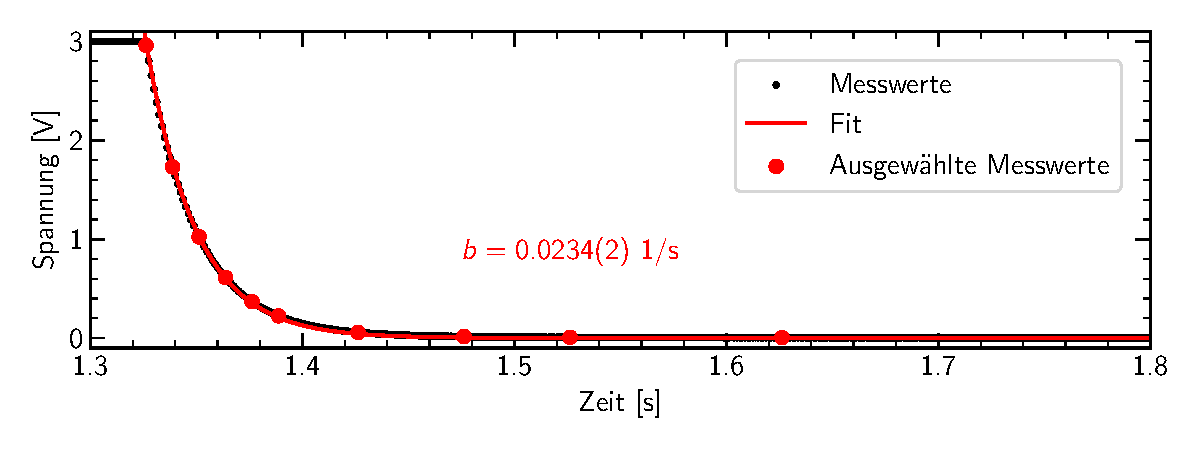
\includegraphics[width=\textwidth]{Versuch7_1}
		\caption{Zeitliche Spannungsdaten während der Kondensatorentladung. In rot wurde die exponentielle Fitfunktion aufgetragen. Die für den Fit herangezogenen Datenpunkte sind ebenfalls rot hervorgehoben. Der Fehler der Spannungsdaten wird nicht dargestellt, dar dieser zu klein.}
		\label{fig:ExpFit}
	\end{figure}

	Die Fitfunktion wurde so gewählt, dass \( \tau_{\text{cap}} = b = 0.0234(2) \unit{1/s} \) gilt und daher Wert und Unsicherheit von Tau direkt vom Fitprogramm berechnet wird. Verwendet man \( \tau = RC \) und setzt Werte für \( R \) und \( C \) ein, erhält man \( \tau_{\text{theo}} = 0.0220(2) \unit{1/s} \). Die Unsicherheit hier kommt nur aus dem Widerstand, da der Kondensator als ideal angenommen wird. Letzteres ist aber normalerweise nicht der Fall, wodurch wahrscheinlich die Diskrepanz zwischen experimentell und theoretisch bestimmten Wert für die Zeitkonstante \( \tau \) rührt.
\end{mybox}

\begin{mybox}{RC Frequenzanalyse}
	\begin{wrapfigure}[19]{r}{4.25cm}
		\vspace{-0.5cm}
		\begin{circuitikz}[european]
			\draw (2.6,0) -- (2,0)
			to[line width=0.3pt, rmeter, t=$U_1$] (0,0)
			to[R, l_=$10 \unit{\ko}$, name=R] (0,4)
			to[rmeter, t=$U_2$] (4,4)
			to[thick, C, l_=$C$] (4,0) -- (3.4,0);
			
			\draw (3,-0.4) to[sV] (3, 0.4);
			
			\draw[latex-, line width=0.5pt] (2.7,0.65) -- (3.3, 0.65);
			
			\node  at (R.center) {$R$};
		\end{circuitikz}
		\caption{RC Schaltkreis mit einem Widerstand  \(  R = 10.0(1) \unit{\ko} \) und einem Kondensator \( C = 2.2 \unit{\micro\farad} \) der an einer Wechselstromspannungsquelle angeschlossen ist. An zwei Stellen wird über einen analogen Port die Spannung aufgezeichnet.}
		\label{fig:2}
	\end{wrapfigure}
	Legt man Wechselstrom an einem Kondensator an, werden Phase und Amplitude der Schwingung verändert, wobei das von der Frequenz der Spannung und den Eigenschaften der elektronischen Komponenten abhängt. Um dieses Verhalten zu untersuchen, wurde ein Schaltkreis mit einem Widerstand  \(  R = 10.0(1) \unit{\ko} \) und einem Kondensator \( C = 2.2 \unit{\micro\farad} \) aufgebaut (Siehe \autoref{fig:2}). Als Wechselstromspannungsquelle wurde mit einem Laptop über ein AUX-Kabel ein Sinusförmiges Signal eingespielt.  
	
	An \( U_1 \) wird die eingespielte Spannung als Referenzmessung aufgezeichnet, während an \( U_2 \) die veränderte Spannung Spannung gemessen wird. Es wurde für Frequenzen \( f = 1, 3, 7, 10, 20 \unit{Hz} \) für 5 Sekunden Daten aufgezeichnet. Unter der Annahme, dass die Frequenz perfekt ist, kennt man auch die Periode \( T = 1/f \) genau und man kann die Schwingungsdaten falten (da das Signal periodisch ist). Sprich man wendet den modulo Operator auf die Daten an und legt \( T-\)sekunden lange Zeitintervalle übereinander (und normiert diese neue Einheitslose Zeitachse von 0 bis 1).
	
	Ob die Faltung erfolgreich war erkennt man daran, dass die Daten bis auf wenige Ausreißer eine schöne Kurve beschreiben. In \autoref{fig:SineFit} sieht man die gefalteten Daten für \( f = 7 \unit{Hz} \) und ohne die Güte zu quantifizieren (z.B. mittels shortest string) würde ich behaupten, dass die Faltung passt. Diese Darstellung hat viele Vorteile, in unserem Fall ermöglicht sie den Fit einer Sinusfunktion der Form \( f(x) = A\sin(\omega x + \phi) \) auf ein langes Zeitintervall, auch wenn die Daten nur Stückweise eine Sinusfunktion beschreiben (da negative Spannungen nicht aufgezeichnet werden). 
	
	\begin{figure}[H]	
		\centering
		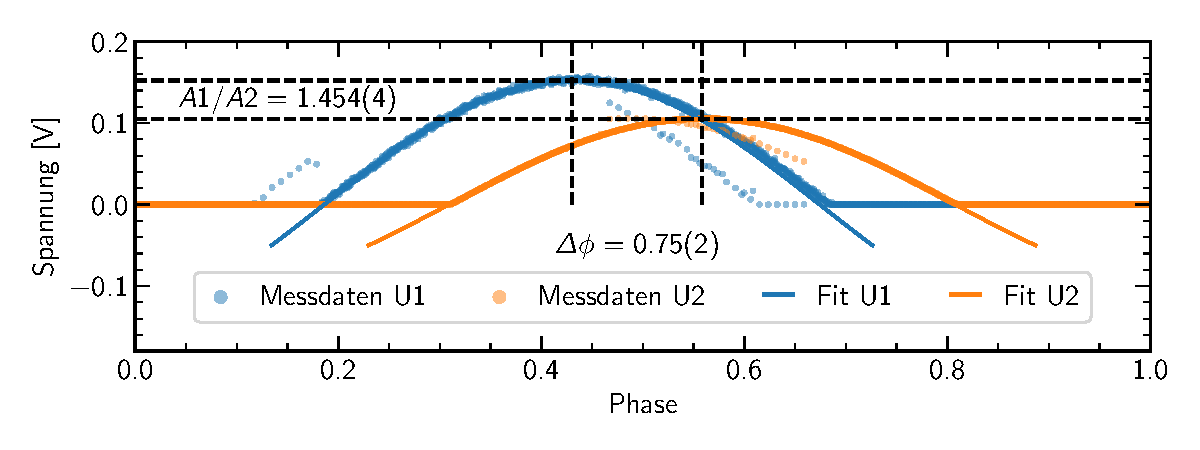
\includegraphics[width=\textwidth]{Versuch7_2}
		\caption{Gefaltete Spannungsdaten für e. In orange sind die Daten der Eingangsspannung und in blau die der Ausgangsspannung aufgetragen. }
		\label{fig:SineFit}
	\end{figure}
	
	Aus dem Fit (und alternativ aus \autoref{fig:SineFit}) lässt sich das Verhältnis zwischen den Amplituden \( A_1/A_2 \) und die Phasenverschiebung \( \Delta\phi = \phi_1 - \phi_2 \) berechnen. Die Fehler ergeben sich aus der Fehlerpropagation der Fehler der Fitparameter. 
	
	Aus dem Skript wissen wir, dass das Amplitudenverhältnis und die Phasenverschiebung mit der Zeitkonstante \( \tau \) wie folgt zusammenhängen:
	\begin{align}\label{eqn:tau2}
		\abs{\frac{A_1}{A_2}}^2 = 1 + (\omega\tau_A)^2 &\quad \Longleftrightarrow\quad \tau_A = \frac{\SQRT{\abs{\tfrac{A_1}{A_2}}^2 - 1}}{2\pi f}\\
		\tan(\Delta\phi) = -\omega\tau_{\phi} &\quad \Longleftrightarrow\quad \tau_{\phi} = -\frac{\tan(\Delta\phi)}{2\pi f}
	\end{align} 
	Wiederholt man die Phasenfaltung und Ermittlung von \( A_1/A_2 \) und \( \Delta\phi \) für \( f = 1, 3, 7, 10, 20 \unit{Hz} \) kann man mittels Gleichungen (2) und (3) einen Wert für die Zeitkonstante \( \tau \) erhalten. In \autoref{table:1} wurden für die 5 Frequenzen die gemessenen Größen und die daraus errechneten Schätzwerte für Tau eingetragen, wobei zwischen 
	
	\begin{center}
		\captionof{table}{Gemessenes Amplitudenverhältnis \( A_1/A_2 \) und Phasenverschiebung \( \Delta\phi \) für verschiedene Frequenzen. Dazu die draus errechneten Werte für \( \tau \).}
		\begin{tabular}{@{\extracolsep{5mm}} 
				r
				S[table-format=1.4(2)]
				S[table-format=1.4(2)]
				S[table-format=1.4(2)]
				S[table-format=1.4(2)]
				S[table-format=1.4(2)]
			}
			\toprule
			\makecell[t]{}
			&   {\makecell[t]{\( 1 \unit{Hz} \)}}
			&   {\makecell[t]{\( 3 \unit{Hz} \)}}
			&   {\makecell[t]{\( 7 \unit{Hz} \)}}
			&   {\makecell[t]{\( 10 \unit{Hz} \)}}
			&   {\makecell[t]{\( 20 \unit{Hz} \)}} \\
			\midrule
			\( A_1/A_2 \) & 1.016(2) & 1.101(2) & 1.454(4) & 1.788(5) & 3.095(15) \\
			\( \tau_{A}\ [1/\text{s}]\) & 0.029(2) & 0.0244(3) & 0.02400(11) & 0.02359(10) & 0.02331(13) \\
			\( \Delta\phi \) & 0.140(11) & 0.483(13) & 0.75(2) & 1.00(2) & 1.29(4) \\
			\( \tau_{\phi}\ [1/\text{s}]\) & 0.022(2) & 0.0278(8) & 0.0211(7) & 0.0247(12) & 0.028(5) \\
			\bottomrule
		\end{tabular}
		\label{table:1}
	\end{center}

	Nun kann man die verschiedenen Messungen für Tau mit einem gewichteten Mittelwert kombinieren und erhält dann \( \tau_{A} = 0.0237(2) \unit{1/s}, \tau_{\phi} = 0.0239(5) \unit{1/s} \). Die Messung der Kondensatorentladung hat einen Wert für die Zeitkonstante von \( \tau_{\text{cap}} = 0.0234(2) \unit{1/s} \) geliefert. Alle drei Methoden zur Abschätzung von Tau sind konsistent miteinander und die Fehler liegen in der gleichen Größenordnung, also können wir die Werte unkompliziert miteinander kombinieren und erhalten somit für die Zeitkonstante \( \tau_{\text{exp}} = 0.0237(2) \unit{1/s} \). Dieser Wert kann nun herangezogen werden, um eine Schätzung für die Kapazität des Kondensators abzugeben, da ja \( \tau = RC \) ist. Setzt man Werte ein erhält man \( C = 2.37(3) \unit{\micro\farad} \).
\end{mybox}

\begin{mybox}{RLC Schwingkreis}
	So wie Kondensatoren, verändern Induktoren die Phase und Amplitude der Schwingung. Um dieses Verhalten zu analysieren, wurde eine Spule mit Induktivität \( L = 100 \unit{mH} \) hinzugefügt. Der Kondensator bleibt unverändert, der Widerstand wurde durch einen mit \( R = 10.0(5) \unit{\ohm} \) ersetzt. Da die zu untersuchenden Frequenzen bei mehreren hundert Hertz liegen, werden am IOLab die \( G_+ \) und \( G_- \) Ports verwendet, da diese eine höhere Abtastrate als die Analogen haben. 
	
	Um das Resonanzverhalten des Schaltkreises zu studieren, wurden wieder über ein AUX-Kabel Sinusförmige Signale eingespielt. Konkret wurden über einen Zeitraum von \( t = 10 \unit{s} \) Sinuswellen zwischen \( 0 \unit{Hz} \) und \( 600 \unit{Hz} \) generiert, wobei die Frequenz linear mit der Zeit zunimmt. Die Idee dahinter war, ein Kontinuierliches Fre
	entweder die Frequenzen über eine Fourier Transformation zu erhalten, oder die Zeitachse durch Frequenzen zu substituieren, da wir die jeweiligen Start- und Endwerte, sowie die Art der Transformation (linear) kennen. Da wir in diesem Versuch für die Analyse nur 10 Datenpunkte hernehmen sollen, wird hier ersteres verwendet. 
	
	In der oberen Grafik in \autoref{fig:Fft} sind die aufgenommenen Spannungsdaten auf die Zeit aufgetragen. Die Schwingungen selbst sind nicht zu erkennen, da die Frequenz zu groß ist. In Orange wurde eine Einhüllende der Daten aufgetragen, aus welcher die Maxima der Schwingungen abgelesen werden können. Es wurden in regelmäßigen Abständen Punkte in der Einhüllenden markiert und an diesen eine Fouriertransformation durchgeführt, welche im unteren Bild dargestellt ist. 
	\begin{figure}[H]	
		\centering
		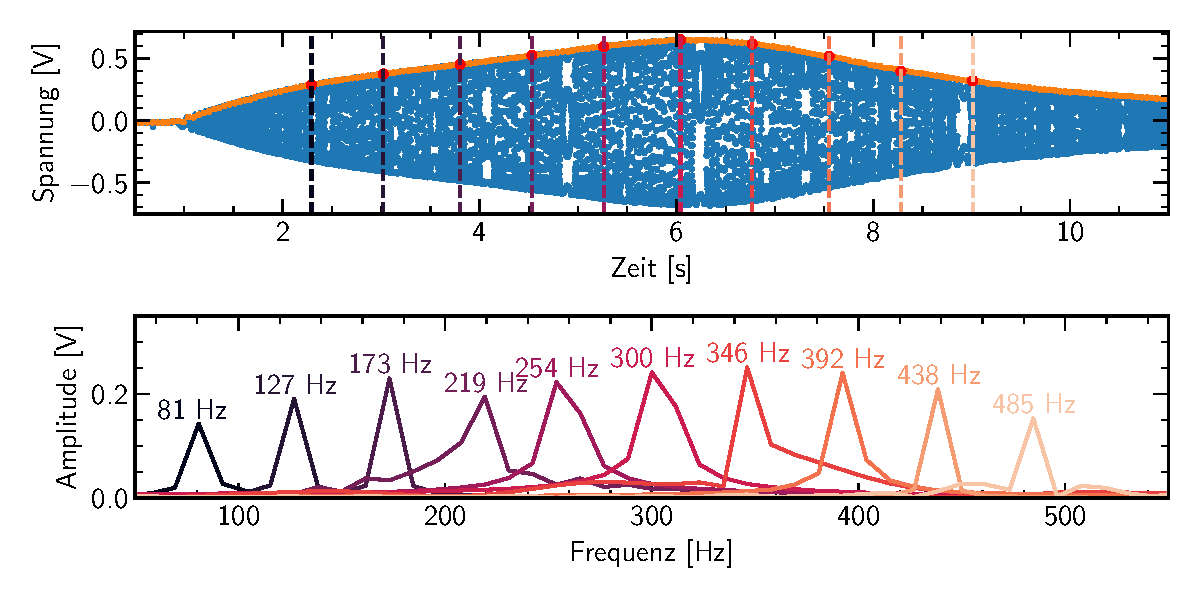
\includegraphics[width=\textwidth]{Versuch7_3}
		\caption{Spannungsdaten für RLC-Schwingkreis bei gleichmäßig zunehmenden Frequenzen von \( 0 \unit{Hz} \) bis \( 600 \unit{Hz} \). In orange ist eine Einhüllende der Daten aufgetragen und in rot wurden Datenpunkte für die weitere Analyse markiert. An den rot markierten Punkten wurde eine Fourier Transformation durchgeführt, welche darunter dargestellt ist.}
		\label{fig:Fft}
	\end{figure}

	Ein Nachteil dieser Vorgehensweise, welcher erst im Nachhinein Auffiel, ist, dass die Abschätzung der Unsicherheit der Maxima nicht trivial ist. Der Fehler der Maxima wurde daher auf den Fehler der Spannungsmessung gesetzt, da sie auf jeden Fall so groß sein müssen, potentiell aber größer sind. Zudem hätte die Fft sehr von einer Messung über ein längeres Zeitintervall profitiert, da die gleiche Frequenz dann für längere Zeit gehalten wird, was zu definierteren Peaks führt. 
	
	Als nächstes wurden die Amplitude der ausgewählten Punkte auf ihre Frequenz aufgetragen. Da es sich hier um Resonanzverhalten handelt, werden die Daten von einer Lorentzfunktion beschrieben, welcher in der Form \( f(x) = \tfrac{A}{\pi} \tfrac{\gamma}{(x-x_0)^2 + \gamma^2} \) an die Daten angepasst wurde. In \autoref{fig:Lorentz} sind 
	
	\begin{figure}[H]	
		\centering
		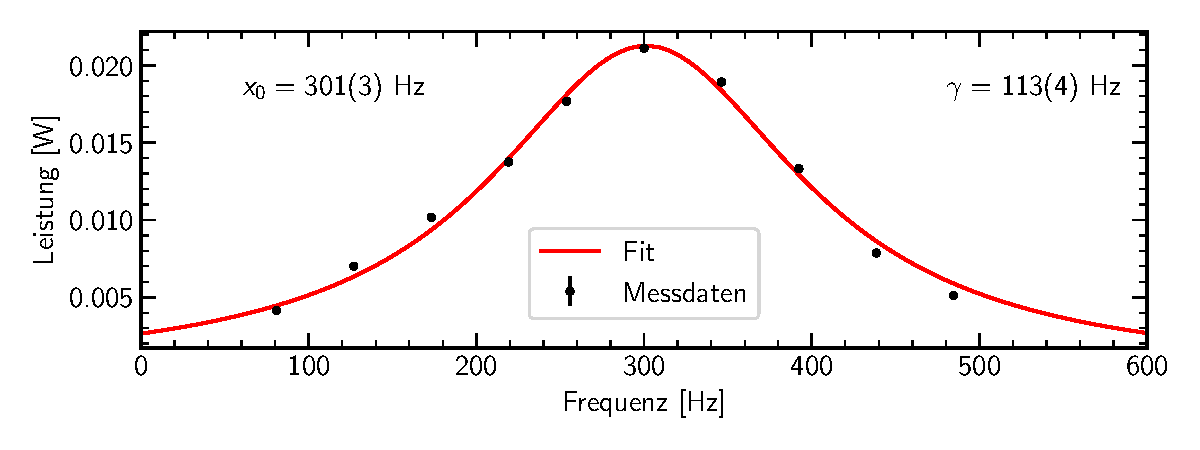
\includegraphics[width=\textwidth]{Versuch7_4}
		\caption{Die am Widerstand umgesetzte Leistung ist für verschiedene Frequenzen dargestellt. In rot wurde eine Lorentzfunktion an die Daten angepasst. Die Resonanzfrequenz \( x_0 \) und die }
		\label{fig:Lorentz}
	\end{figure}

	Aus dem Lorentz Fit lässt sich direkt die Resonanzfrequenz \( f_{\text{res}} = x_0 = 301(3) \unit{Hz} \) und die Bandbreite \( \Delta f = 2\gamma = 227(9) \unit{Hz} \) herauslesen. Die Resonanzfrequenz lässt sich auch theoretisch bestimmen und ist gegeben durch 
	\begin{equation}\label{eqn:fres}
		f_{\text{res}} = \frac{1}{2\pi\sqrt{LC}}
	\end{equation}
	. Setzt man nun \( C = 2.37(3) \unit{\micro\farad} \) und \( L = 100 \unit{mH} \) in \autoref{eqn:fres} ein, erhält man \( f_{\text{res}} = 327(2) \unit{Hz} \). Dieser Wert ist zwar so nicht mit dem experimentell bestimmten vereinbar, die Größenordnung ist aber die gleiche und wie weiter oben angemerkt sind die Fehler für die Spannungswerte zu klein abgeschätzt. Die Bandbreite brauchen wir, um die Güte \( Q \) des Schwingkreises zu bestimmen. Diese ergibt aus 
	\begin{equation}\label{eqn:Q}
		Q = \frac{1}{R}\SQRT{\frac{L}{C}} = \frac{f_{\text{res}}}{\Delta f}
	\end{equation}
	. Wieder setzen wir Werte für \( R, C \) und \( L \) ein und erhalten als einen Theoriewert zum Vergleichen \( Q = 20.6(1.0) \). Teilen wir aber die experimentell bestimmte Resonanzfrequenz durch die Bandbreite erhalten wir \( Q = 1.33(5) \). Diese Abweichung ist hochsignifikant und lasst sich nicht durch zu klein abgeschätzte Fehler erklären. 
\end{mybox}


\end{document}